%%%%%%%%%%%%%%%%%%%%%%%%%%%%%%%%%%%%%%%%%%%%%%%%%%%%%%%%%%%%%%%%%%%%%%%%%%%%%%%%
%2345678901234567890123456789012345678901234567890123456789012345678901234567890
%        1         2         3         4         5         6         7         8

\documentclass[letterpaper, 10 pt, conference]{ieeeconf}  % Comment this line out
                                                          % if you need a4paper
%\documentclass[a4paper, 10pt, conference]{ieeeconf}      % Use this line for a4
                                                          % paper

\IEEEoverridecommandlockouts                              % This command is only
                                                          % needed if you want to
                                                          % use the \thanks command
\overrideIEEEmargins
% See the \addtolength command later in the file to balance the column lengths
% on the last page of the document



% The following packages can be found on http:\\www.ctan.org
\usepackage{graphics} % for pdf, bitmapped graphics files
\usepackage{epsfig} % for postscript graphics files
\usepackage{mathptmx} % assumes new font selection scheme installed
\usepackage{times} % assumes new font selection scheme installed
\usepackage{amsmath} % assumes amsmath package installed
\usepackage{amssymb}  % assumes amsmath package installed
\usepackage{cite}  % for easy citing outputs
\usepackage{color}

\long\def\dv#1{\textcolor{red}{**[DV] #1**}}
\long\def\zt#1{\textcolor{green}{**[ZT] #1**}}

\usepackage[caption=false,font=footnotesize]{subfig}
\usepackage{algorithmic}
\usepackage{algorithm}
\pdfminorversion=4

\title{Uncertainity Based Human Aware Navigation}



\author{Zeynab Talebpour$^{1}$ \and Deepak Viswanathan$^{2}$ \and Rodrigo Ventura$^{3}$ \and Alcherio Martinoli$^{4}$% <-this % stops a space
\thanks{$^{1,4}$Distributed Intelligent Systems and Algorithms Laboratory,
School of Architecture, Civil and Environmental Engineering,
 \'Ecole Polytechnique F\'ed\'erale de Lausanne 
        {\tt\small \{zeynab.talebpour, alcherio.martinoli\}@epfl.ch}}% <-this % stops a space
\thanks{$^{2}$Deepak Viswanathan, Department of Informatics, University of Amsterdam
        {\tt\small D.geethaviswanathan@uva.nl}}%
\thanks{$^{3}$Rodrigo Ventura, Institute for Systems and Robotics, Instituto Superior T\'ecnico, Universidade de Lisboa, Portugal
        {\tt\small  rodrigo.ventura@isr.ist.utl.pt}}%
\thanks{This research was supported by the European MOnarCH project FP7-ICT-9-2011-601033.}%
}

\begin{document}



\maketitle
\thispagestyle{empty}
\pagestyle{empty}


%%%%%%%%%%%%%%%%%%%%%%%%%%%%%%%%%%%%%%%%%%%%%%%%%%%%%%%%%%%%%%%%%%%%%%%%%%%%%%%%
\begin{abstract}
%In this work, we present a novel approach to human-aware navigation based on the fast marching method, by probabilistically modeling the uncertainty in on-board perception components of a social robotic system and investigating its effect on the overall social navigation performance. We have extended the model of the social costmap around a person to consider this new uncertainty factor which plays an important role in situations with noisy perception. Real robot experiments have been carried out to show the effectiveness of our approach in realistic scenarios with noisy perception involving a single dynamic human. Results show how our approach has been able to achieve trajectories which are more socially-aware compared to the basic navigation approach, and the human-aware navigation approach which relies solely on perfect perception.
In this work, we present a novel approach to human-aware navigation based on the fast marching method, by probabilistically modelling the uncertainty of perception for a social robotic system and investigating its effect on the overall social navigation performance. We have extended the model of the social costmap around a person to consider this new uncertainty factor which plays an important role in situations with noisy perception.  
Real robot experiments have been carried out to show the effectiveness of our approach given noisy perception, in the presence of single/multiple, static/dynamic humans. Results show how our approach has been able to achieve trajectories which are more socially-aware compared to the basic navigation approach, and the human-aware navigation approach which relies solely on perfect perception.In extensive experiments carried out with real robots and
in simulation we demonstrate the performance of our approach.


\end{abstract}


%%%%%%%%%%%%%%%%%%%%%%%%%%%%%%%%%%%%%%%%%%%%%%%%%%%%%%%%%%%%%%%%%%%%%%%%%%%%%%%%
\section{Introduction}

\dv{Need to have 6 paragraph. 
First para stays. \\
Second should motivate human aware navigation using FMM. This means motivating FMM and then human aware navigation using FMM. Also in this para, mention about global and local path planning stategies.\\ 
Next para should be about the social cost map using proxemics.(I prefer this order since social cost map can only be mentioned after you explain the framework (FMM or DWA which is the path planner).\\
4th para seems ok now. We motivated social path planning using social cost maps and planners like FMM or DWA. In this para we talk about how and why uncertainity should be used.\\
5th para is the place where we talk about our two models.\\
6th Para should be our results. "We also show from our experiments that...global path planning has these positives and negatives when used for real human aware planning using uncertainity, whereas local strategies have these these issues. }

\dv{Motivating our work in one para. Looks good for now}
Human aware navigation is a key problem in social robotics. If robots need to be actively used in natural social environments, one of the main components required is navigation. Robust navigation principles incorporating humans in the environment need to be developed. Robots have to navigate in environments shared with humans and the quality of their movement strongly influences  how their intelligence is perceived~\cite{Althaus2004}. Conventionally, comfort, naturalness and scalability, are the main focus of such human aware navigation techniques ~\cite{Kruse2013}. In this work, we attempt to model one essential aspect of human aware navigation which has been overlooked in this area, uncertainty in the perception.

\dv{How do we do human aware navigation. We do it by using social costmaps fed into a navigation planner. So first talk about the path planning, I think we should say that people have tried to do this using global planners. And also talk about local planners. Add a para here about social path planners.}

One important concept which is used in numerous studies~\cite{Mumm2011,Takayama2009,Walters2011,ferrer2013robot} in this area is virtual space around a person that is mutually respected by other humans, called \textit{proxemics}~\cite{Hall1969}.
Based on this concept, depending on the relationship and the interaction that exists between humans, people choose different social distances relating to intimate, personal, social or public contexts.
Changes in the expected distance may indicate dislike if it is too large or cause discomfort if it is too small.\dv{avoid ideas like these. This has no relavance to our story} 


Social costmaps are a common way to model this principle and have been used in various studies in the field. There are many factors that have a role in shaping this costmap, but the proxemics distance is mainly addressed. Other factors such as speed of a person's movement, gender, age, etc. have also been considered in the literature, but are much less common.\dv{This way of phrasing the available works, makes it feel like uncertainity is just another factor that people ignored to consider. we need to rephrase this idea of social cost maps} 

%To the best of our knowledge, there does not exit any work on including uncertainty of perception in this problem. If the center of the costmap, which indicates the position of the person in not deterministically known, the costmap can not correctly model the social costs and hence the social path planning could fail in finding an appropriate socially compliant path. This problem becomes much more critical in real applications where robustness is vital for succeeding under different conditions.  

%Robots will progressively become part of the work spaces and habitats of humans.Despite where they are located, in home environments or hospitals as assistants, in factories as co-workers or as guides in supermarkets, a key behavior which they all share is navigation.Robots have to navigate in environments shared with humans and the quality of their movement strongly influences  how their intelligence is perceived~\cite{Althaus2004}. Consequently, new methods for robot navigation in the presence of humans are being studied extensively. Kruse et al.~\cite{Kruse2013} present a thorough survey of such methods where they identify comfort, naturalness and scalability as the three key issues addressed by the existing human-aware robot navigation methods so far. %(last 2 sentences taken from  RV's paper)
%Hence socially-aware navigation which pays special consideration to people 


%Presence of humans in an environment should be properly perceived by a robot as a requirement for a socially-aware path planner that takes into consideration individual humans and possible social interactions taking place in the environment. This information can be obtained by an external source such as an overhead camera or can be attained using on-board sensors of the robot. while there are advantages and disadvantage to both cases, on-board perception allows for a fully autonomous and independent robot that relies only on itself for taking decisions about the world. Moreover, there are environments which do not permit the use of external infrastructures required for providing the requisite perception, due to reasons such as privacy or security issues or etc. Therefore, providing the required perception for human-aware navigation with on-board sensors is a desirable characteristic for a robot which helps integration of such systems into real-world environments.  \dv{This paragraph is irrelavant to motivating our work. lets stick with only the story of uncertainity in perception}

%Presence of humans in an environment should be properly perceived by a robot as a requirement for a socially-aware path planner that takes into consideration individual humans and possible social interactions taking place in the environment. However, perception will never be perfect and is affected by various elements such as the movement of the robot, movement of the person, complexity of the environment in terms of occlusions, etc. Due to the approximate nature of the models and the less than perfect detectors available, we often can only provide estimate of location of the people with significant uncertainty. Any planning algorithm which needs to rely on real perception sources must be able to use this less than perfect estimates. The assumption of having perfect information about the position and orientation of people at all times, is common in the state of the art research in this area, where the main focus is on the planning itself. However, moving to real applications, poses serious challenges in terms of noisy perception information and high uncertainties, that need to be addressed and modeled in a human-aware approach.

\dv{By the time we are here, we should get the idea about social cost map clear, socially aware path planner clear. then the next para makes sense.}
A socially-aware path planner should take into consideration individual people and possible social interactions taking place between the people in the environment. However, perception will never be perfect and is affected by various elements such as the movement of the robot, movement of the people, complexity of the environment in terms of occlusions, etc. Due to the approximate nature of the models and the less than perfect detectors available, we often can only provide estimate of location of the people with an associated uncertainty. Any planning algorithm which needs to rely on real perception sources must be able to use this less than perfect estimates. The assumption of having perfect information about the position of people at all times, is common in the state of the art research in this area[ref][ref] \dv{must add references}, where the main focus is on the planning itself. However, moving to real applications, poses serious challenges in terms of noisy perception information and high uncertainties, that need to be addressed and modeled in a human-aware approach.


%Different perception sources for person detection and tracking, have different levels of uncertainty and accuracy in their detections. while, there exist trackers able to perform this task with cm-level accuracy, others have a much larger uncertainty associated to them. If a human-aware approach, could take this into account, the same planning method could easily be reused even when the source of perception changes. As an example while overhead cameras can provide position information of people with good accuracy, when moving to on-board perception for a mobile robot, this accuracy and the associated uncertainty will largely change. This is even more significant, if tracking is done using an ultra-wide-band (UWB) tag. So, for more robustness and effectiveness, a human-aware navigation method, should be able to handle all these situations without undergoing major changes. This is possible, by adaptively changing the social costs.\dv{This para is kind of redundant. Does not add much value to generalize our work. In discussions and possible extentions we can mention how to generalize our work. Definitely not in introduction}

%However, perception will never be perfect and is affected by various elements such as the movement of the robot, movement of the person, complexity of the environment in terms of occlusions, etc. Unlike other works which choose to ignore this very important aspect of the uncertainty in perception, we propose a model which computes the uncertainty of the location and orientation of the people in an environment. We aim to study, how this factor should influences the social costs used by the path planner and how taking this into account the resulting trajectories will be improved in terms of social acceptability.

%\dv{Discussion of proxemics makes it harder to follow the narrative. Need to restructure the introduction from here on. The story is broken. first two paragraphs motivated human aware navigation and real perception systems. what now? how do you think we should continue the story? - i am unclear on this. how does proxemics fit into the narrative? transition lines are very important which connect the story.}



%\dv{again. this paragraph needs to be worked on. I don't think we should suddenly switch to human robot interaction. thats not what this paper is dealing with. Uncertainity in human aware navigation. thats all we care about.}
%As stated in~\cite{gomez2013social}, recent work in the human-robot interaction domain can be divided in three categories of 1) human-robot proxemics, 2) human-aware planning and navigation, and 3) robot-to-human approaching and behaving. In this work we focus mostly on the second category using the concepts from human-robot proxemics. %Human-aware path planning has been an area of interest particularly in the recent years. 

\dv{Core idea for last para}
In this work, we have developed a human aware navigation method incorporating uncertainity in perception. By using an FMM based social navigation planner and a DWA based social navigation planner, we compare how a global and local planning strategy can be used for human aware navigation. We explore the benefits of each strategy in a stochastic environment with varying uncertainity about the location of the people in the environment.

\dv{Use all you need from below for the FMM and DWA para. but all details should be pushed to background. Introduction should be crisp and clear.}

In this research we are introduce a novel social path planning approach based on the fast marching method (FMM)~\cite{sethian1999fast}. FMM has been proven to be successful in real domestic spaces with high complexity\cite{ventura2015}. However, we add a social component to the aforementioned method by augmenting it with social costmaps \textemdash based on proxemics principles~\cite{kirby2009companion}\textemdash~around around individual people which correspond to speedmaps for the FMM method. %\dv{next line should be pushed to background}%
There have previously been a number of research papers which have address social path planning~\cite{gomez2014fast,gomez2013social} using FMM. %However, their model is based on known person position and orientation in simulation. 

%\dv{needs more work.}
The work of ~\cite{gomez2014fast} a theoretical framework for introduced sub-problems of social path planning is presented and an extended mode for engaging groups of people is proposed by using a special version of fast marching square planning method~\cite{valero2013fast}. Nonetheless, the information about humans are considered to be given and noiseless, while only simulations have been used to show the effectiveness of the proposed method for static people. We are interested in investigating the same problem in real-world scenarios with the challenges that exist therein. Particularly, in the case of moving people, while the perception is subject to uncertainty. 
%We believe that uncertainty of perception in social robotics is an important topic which to our knowledge is very little explored.
We believe that uncertainty of perception in social robotics, is an important topic which to our knowledge, has not been the subject of many notable studies. There is a dedicated chapter in \cite{correa2014uncertainty} on local planning with uncertainty, however this is not considered in a social context. The sources of uncertainty in~\cite{correa2014uncertainty} are the position of the robot and the obstacles, and the partially known motion of moving obstacles and perception of people and the uncertainty in person and group detection and tracking has not been investigated.

Another interesting aspect of human-aware navigation problem which should be deeply investigated is knowing how to decide when to replan. As a perquisite, We have studied whether accounting for social costs in the local planner can be effective. In basic navigation, the global path planner, provides a plan and local planner deals with dynamic obstacles and collision avoidance for making it possible to reach the goal. It is common to have social path planners considerate of people's presence and activities, but this is seldom taken into account for local path planners. Of course, this reactive short horizon control does not exactly have a social nature but it is interesting to see, how accounting for social costs in this low level is reflected on the higher level navigational behavior of the robot. By delegating part of the work to the local planner, the cost of global planning which is much larger than the local planning can be reduced. However, for the best behavior, a hybrid approach that adopts the use of social planners on both level is more effective.    

The remainder of this article is organized as follows. In section~\ref{sec:background} we introduce the background for this work. Section~\ref{sec:algorithms} explains the methods and models. In section~\ref{sec:results}, we show the results of our simulations and real robot experiments and finally, section~\ref{sec:conclusion} concludes this work.

%\paragraph{Story}  - Quantify uncertainity in perception. Use this for generating cost maps adaptively. FMM creates plans using this uncertainity model.



%\dv{Modelling and accurately computing the location and orientation of a person in an environment is a hard problem. Typically, in state of the art people tracking methods, a bayesian approach is used.}


% \paragraph{Motivation and approach} - Perception will never be perfect. Unlike other works which choose to ignore this very important aspect of the uncertainty in perception, we propose a model which computes the uncertainty of the location and orientation of multiple people in an environment. We use this model to make informed choices about the cost function for navigation which is then used by a state of the art navigation model using FMM. We dynamically replan based on the perception information available. The key idea is that in cases where the perception is unreliable, we need to make sure that the robot navigates prioritizing safety over social norms.

% paragraph{Note} Active perception is also important. The robot movement causes uncertainty which can be actively reduced by taking paths which improve the perception information.



%\subsubsection{Additional Stuff}
%However, contrary to approach we propose in this paper, these works are only validated in computer simulation.Comfort is defined as a relative state in which the body is relieved of unpleasant sensory or environmental stimuli [25]
\section{Background}
\label{Literature}
%In this research we are introduce a novel social path planning approach based on the fast marching method (FMM)~\cite{sethian1999fast}. 
%\dv{Place our work. Use this section as a narrative to place our work among the available works on human aware navigation. By the end of this section it should be clear how and why our work is relavant. Coarse overview :Broadly summarize the works on human aware navigation historically. Then come to introducing FMM and its use in human aware navigation. One para about local planning (DWA) and its applicability in human aware navigation. One para about people tracking works and probabilsitc model.}


Human-aware navigation focuses on the interaction dynamics between humans and robots that occur as a result of navigation~\cite{Kruse2013}. 
In the literature, we can find several strategies for comfort ranging from appropriate approaching strategy~\cite{Dautenhahn2006}, maintaining appropriate distance~\cite{Takayama2009}, control strategies to avoid being noisy~\cite{Martinson2007} and use of planning for avoiding interference~\cite{Vasquez2012}. In this work we focus on the principle of proxemics which is the most common in the literature of human-aware navigation, with social costs encoded as costmaps similar to~\cite{gomez2013social} along with an FMM-based path planner.



FMM has been proven to be successful in real domestic spaces with high complexity\cite{ventura2015}. There have previously been a number of research papers addressing social path planning~\cite{gomez2014fast,gomez2013social} using FMM. %However, we add a social component to the aforementioned method by augmenting it with social costmaps \textemdash based on proxemics principles~\cite{kirby2009companion}\textemdash~ around individual people which correspond to speedmaps for the FMM method. %\dv{next line should be pushed to background}%
 %However, their model is based on known person position and orientation in simulation. 
%\dv{needs more work.}
In the work of~\cite{gomez2014fast} a theoretical framework for introduced sub-problems of social path planning is presented and an extended model for engaging groups of people is proposed by using a special version of fast marching square planning method~\cite{valero2013fast}. Nonetheless, the information about humans are considered to be given and noiseless, while only simulations have been used to show the effectiveness of the proposed method for static people. We are interested in investigating the same problem in real-world scenarios with the challenges that exist therein. Particularly, in the case of moving people, while the perception is subject to uncertainty. 
%We believe that uncertainty of perception in social robotics is an important topic which to our knowledge is very little explored.



We believe that uncertainty of perception in social robotics, is an important topic which to our knowledge, has not been the subject of many notable studies. There is a dedicated chapter in \cite{correa2014uncertainty} on local planning with uncertainty, however, this is not considered in a social context. The sources of uncertainty in~\cite{correa2014uncertainty} are the position of the robot and the obstacles, and the partially known motion of moving obstacles, perception of people and the uncertainty in person and group detection and tracking has not been investigated.

%Another interesting aspect of human-aware navigation problem which should be deeply investigated is knowing how to decide when to replan. As a perquisite, We have studied whether accounting for social costs in the local planner can be effective. In basic navigation, the global path planner, provides a plan and local planner deals with dynamic obstacles and collision avoidance for making it possible to reach the goal. It is common to have social path planners considerate of people's presence and activities, but this is seldom taken into account for local path planners. Of course, this reactive short horizon control does not exactly have a social nature but it is interesting to see, how accounting for social costs in this low level is reflected on the higher level navigational behavior of the robot. By delegating part of the work to the local planner, the cost of global planning which is much larger than the local planning can be reduced. However, for the best behavior, a hybrid approach that adopts the use of social planners on both level is more effective.    

\zt{Deepak please add background for tracker}
\section{Experiments}
\label{exp}
In this section we will briefly explain our robotic platform, experimental setup and the set of experiments along with the metrics which have been conducted to evaluate the performance of our system.

\subsection{Robotic Platform}
\label{sec:robot}

\begin{figure}
\centering
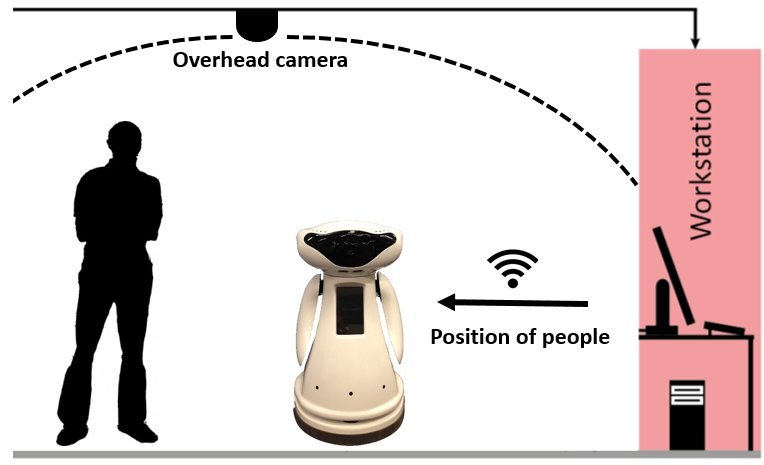
\includegraphics[width=0.4\textwidth]{pictures/setup.jpg}\label{fig:robot}%
\caption{Experimental setup schematics and the MBot robotic platform.}
\label{fig:setup}
\end{figure}

%\begin{figure}
%\centering
%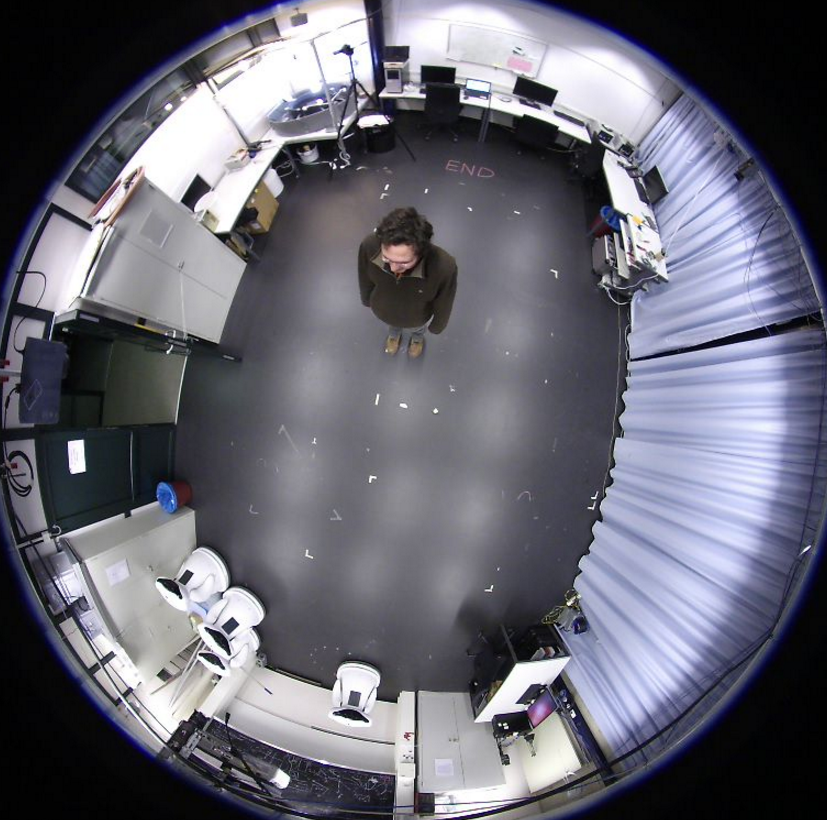
\includegraphics[width=0.3\textwidth]{pictures/arena.png}\label{fig:arena}%
%\caption{Experimental arena. The robot starts from its initial position and navigates to the end point while dealing with the people in the environment. This is a snapshot of the first step of the single static person case.}
%\label{fig:setupArena}
%\end{figure}


%\begin{figure}
%    \centering
%    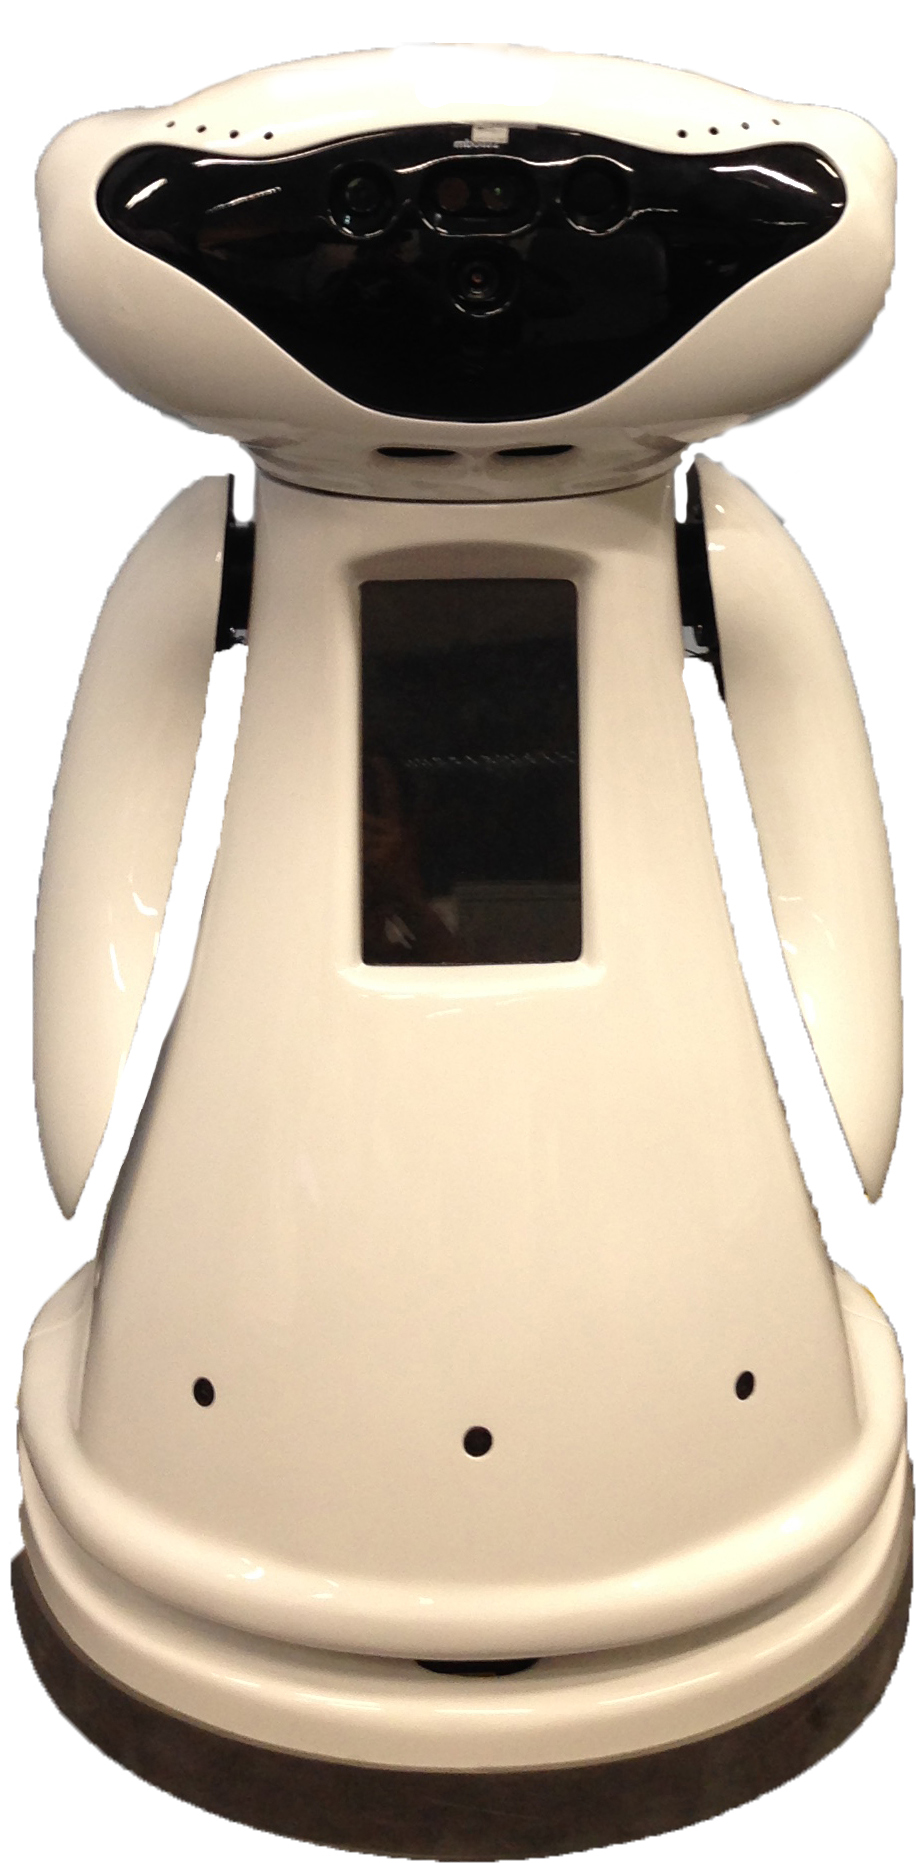
\includegraphics[scale=0.07]{pictures/robot.jpg}
%    \caption{Robot used in our experiments to perform the automatic fingerprinting.}
%     \label{robot}
%\end{figure}


The robotic platform used in this work is shown in Fig. \ref{fig:setup}. This robot is called MBot \cite{Messias2014robotic} and is developed within the FP7 European project MOnarCH.
It is an omni-directional drive robot with an approximately round footprint of 0.65~\textit{m} in diameter and a height of 0.98~\textit{m}.
It is provided with two laser range finders, on both the front and the back for providing 360$^{\circ}$ coverage.

Two batteries give it an autonomy of approximately five hours, depending on the usage.
The robot has two PCs inside its shell: one manages the sensors, navigation and actuators, while the second one is for other functions such as human-robot interaction functionalities.%, which are outside our interests for this work.
 The two on-board PCs, run Ubuntu desktop 12.04 and ROS Hydro. 


\subsection{Experimental Setup}
\label{sec:Experimental_setup}

We have used an extensive suite of experiments both in simulation and reality, for performance evaluation. A high fidelity robotic simulator Webots \cite{michel1998webots}, with realistic models of the MBot and the testing environment has been used for evaluations in the initial step. The trackers have been emulated initially, but real recorded data bags of perception were used in the next steps for more close to reality simulations. This was done to simplify the debugging process and speeding up the robotic experiments. %by replaying real uncertainty and tracking data from real experiments.
Finally, we tested our methods in reality in three different scenarios, in a laboratory environment of 5~\textit{m}~$\times$~7~\textit{m}%, depicted in Fig. \ref{fig:arena} 
~where the tracker was operational.
 
%\begin{figure*}[t]
%\centering
%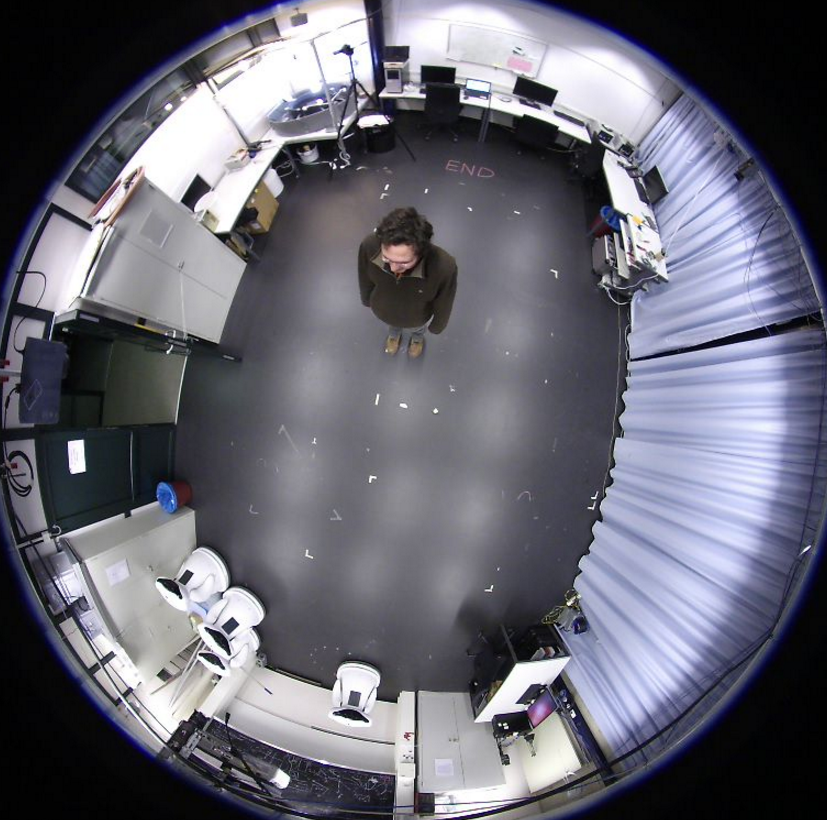
\includegraphics[width=0.30\textwidth]{pictures/arena.png}
%\caption{Connection of different system components.} %The social navigation layer adds the costs associated to people to other costmaps for taking path planning decisions.}
%\label{fig:arena}
%\end{figure*}

We used a networked omnidirectional overhead camera with a field of view of 180$^{\circ}$, to track the positions of the people in the environment. This type of camera was chosen because: (1) it is less obtrusive, and can be left in the environment with less risk of making people feel uncomfortable about being watched; 
(2) it provides a global view of the area, with lower risk of occlusion than elevated side-view cameras and with more flexibility as to its positioning; (3) the number of cameras needed in the environment can be reduced, which has benefits in terms of equipment cost, installation cost and computational load of the perception algorithms. 


%People detection and tracking is done by means of a networked omni-directional cmaera with 180 degrees field of view. 
The tracker outputs results at the rate of 3~\textit{Hz}. The ground truth position of the robot is given by AMCL with 5-10~\textit{cm} accuracy, and the person stands and walks on physically marked tracks to get the exact precise ground truth for the purpose of performance evaluation.
The control rate of navigation is 20~$Hz$ while the social costmap generation has a rate of approximately 3~\textit{Hz}. This is to account for the low output frequency of the tracker.


\subsection{Scenarios}
\label{sec:scenarios}

We have studied three different scenarios, each having been tested five times. We started with 1) a single static person and incrementally increased the complexity to 2) one moving person and finally, 3) two static people in the arena. It should be emphasized that perception uncertainty is affecting the tracking performance and is not evident or quantifiable from just looking at the environment. This means, the person is not aware of what is happening on the tracker side, however, the information given by the tracker greatly affects the behavior of the robot, and therefore the social acceptability. 


Since we aim to study the effect of perception uncertainty in human-aware navigation, we chose a task of point to point navigation for the robot in the vicinity of humans, which is the most general and basic navigation task.

%The complexity of the navigation task can be increased and more interesting scenarios in terms of Human Robot Interaction (HRI) can be investigated, but that is outside the scope of this work. 

In each experiment, the robot starts from a predefined starting point and is sent to one predefined goal. The robot then has to behave appropriately when it encounters people in the arena. For the static case, there is always a person standing between the robot and the straight line to the goal, and for the dynamic case the person moves along this line in the opposite direction, as the robot starts navigating towards the goal, causing a direct encounter with the robot. The following section will explain the metrics used for performance assessment.% in our experiments.

%
%Figure shows a snapshot of the setup with two people moving in the arena. For the case of static people we have also done extensive tests using a high fidelity simulator webots \cite{michel1998webots}, by 1) emulating the uncertainty of tracking, and 2) replaying real uncertainty and tracking data from real experiments. 


\subsection{Metrics}

Five different metrics have been defined for performance evaluation. A subset of these metrics is chosen for each experiment based on the scenario of interest.% Table \ref{table:metrics} briefly describes each of the metrics and the scenarios they have been used for.

\begin{itemize}[ noitemsep, leftmargin=*]

\item $m_{1}$: Measures the minimum distance that the robot has kept during the experiment to a human.% If this distance is not large enough, the robot will be invading the personal space of the person and will therefore cause discomfort. 


\item $m_{2}$: Evaluates how long the robot has been moving in areas associated with social costs, \textit{i.e.}, a position with corresponding non-zero value in the costmap.

\item $m_{3}$: Quantifies the accumulated social cost, this is to differentiate between being in different positions of the social costmap, which is not reflected in $m_{2}$. So if the robot is closer to a person, the social cost will be higher and this metric will increase. For more information on $m_{1}-m_{3}$ refer to \cite{talebpour2015board}. 

\item  $m_{4}$: Evaluates the smoothness of the robot trajectory. This is important from the human observer's point of view when perceiving the robot motion. Humans are known to prefer motion with minimum jerk \cite{sisbot2010synthesizing}, therefore we took the root mean squared error (RMSE) of the trajectory jerk in $m_{4}$:
\begin{equation}
r_{t} = \begin{bmatrix}
x_{t}\\
y_{t} 

\end{bmatrix} \, , \, \,  
%m_{4} = \sqrt{\frac{1}{N} \sum_{t=1}^{N}\left | \dddot{r_{t}} \right |^{2}  }
m_{4} = \sqrt{\frac{1}{N} \sum_{t=1}^{N}\left | \frac{\mathrm{d^3} r_{t} }{\mathrm{d} t^3} \right |^{2}  }
\end{equation}


$r_{t}$ indicates the position of the robot at time $t$, and $N$ indicates the total time of the experiment. It should be emphasized that we did not actively try to modify the robot control to get smoother trajectories, we are just interested to see which method results in a more natural and smooth path.  

\item $m_{5}$: Is the total time steps required to finish the navigation.% task.


%\item $m_{6}$: Measures the minimum of the average distance of the robot to all the people present in the environment. This is interesting since it shows how the robot is choosing to use the space. Does it choose to go through the area between the people or does it prefer to take a tour and increase this minimum average distance?

\end{itemize}

%\begin{table}[h!]
%\centering
%\begin{tabular}{||c l c||} 
 %\hline
 %Name & Description & Scenario \\ [0.5ex] 
 %\hline\hline
 %$m_{1}$ & Minimum distance to a person (\textit{m}) & 1,3 \\ 
 %$m_{2}$ & Time steps spent in areas with social cost & 1,3  \\
 %$m_{3}$ & Accumulated social cost & 1,3  \\
 %$m_{4}$ & Smoothness of the trajectory & 1,2,3  \\
% $m_{5}$ & Time steps to finish the task & 1,2,3  \\
 %$m_{6}$ & Minimum average distance to the people (\textit{m}) & 3  \\ [1ex] 
% \hline
%\end{tabular}
%\caption{Performance metrics.}
%\label{table:metrics}
%\end{table}



\section{PROBABILISTIC TRACKING MODEL}
We are interested in the underlying \textit{state} of the environment which is modelled as a tuple: location and orientation of the people. The \textit{discriminative detectors} used to estimate these state variables have associated noise due to various state factors such as occlusion, lighting conditions, different posture of people, motion of the robot and the people. Coupled with this, there is also stochasitcity in the state transitions, which makes it hard to compute an exact estimate of the location of the people. A principled approach to solve this problem, is to compute a \textbf{belief} (posterior distribution) over the states using recursive bayesian estimation. More formally,

LeT $\textbf{X}_{t}$ be the state of the environment at time \textit{t}.
\begin{align}
P(\textbf{X}_{t} | \textbf{O}_{t}) = \dfrac{P(\textbf{O}_{t} | \textbf{X}_{t}) P(\textbf{X}_{t}|\textbf{X}_{t-1})} {P(\textbf{X}_{t-1})}
\end{align} 

Where, $P(\textbf{O}_{t} | \textbf{X}_{t})$ is the likelihood of the state given all our observations (detector outputs). Computation of this likelihood is best performed by using a learnt model of how the detectors perform for different states. Details of how these \textit{observation models} are created is explained in the next section.

$P(\textbf{X}_{t}|\textbf{X}_{t-1})$ is the \textit{transition model} which models the evolution of the state variables. For a multi person natural environment, an exact analyitical model is intractable. We model the motion of the people independently. we assume a first order model for motion incorporating velocity of the person. Interactions between people are environment specific and is outside the scope of this work. So we choose to ignore this aspect of the environment and attribute it to the uncertainity we have in the state estimation. The exact model for a multi person environment is given in section ......

Another important aspect is the computation of this belief itself. the state space is extremely complex so as to compute exactly this probability 
distribution over the states. We use an MCMC based sampling algorithm to approximately compute the belief. The details of our sampling alogorithm is given in section .......

%For the purpose of the human aware navigation planner, we transform these beliefs to a lower dimensional representation which is a 2-dimensional gaussian over the location of the person.

\subsection{Detector}
We use a probabilsitic background based detector
\subsection{Observation models}
We learn from data, the distribution $P(\textbf{O}|\textbf{X})$ for each detector. 


\section{Results and Discussion}
\label{res}
%Need to explain the experimental set up here. Omnidirectional camera, monarch platform. And motivating the experiments below. 
%\dv{Need to identify one or two scenarios where the uncertainity will help us. Like two people standing close by and the robot not going in between them. In the other case with deterministic tracker, the robot should go in between them.}\\

For each of the scenarios described in Section \ref{sec:scenarios}, we have compared the results obtained from the Basic Navigation (BN), Deterministic (DHA), K-means clustering (KHA), mean Shift clustering (SHA), and social cost Convolution (CHA) Human-Aware (HA) navigation. We will only report the trajectories and metrics obtained from the results of our real experiments for the sake of conciseness. Larger values for $m_{1}$, and smaller values for $m_{2}$-$m_{5}$ are preferable.


\begin{figure}
\centering
{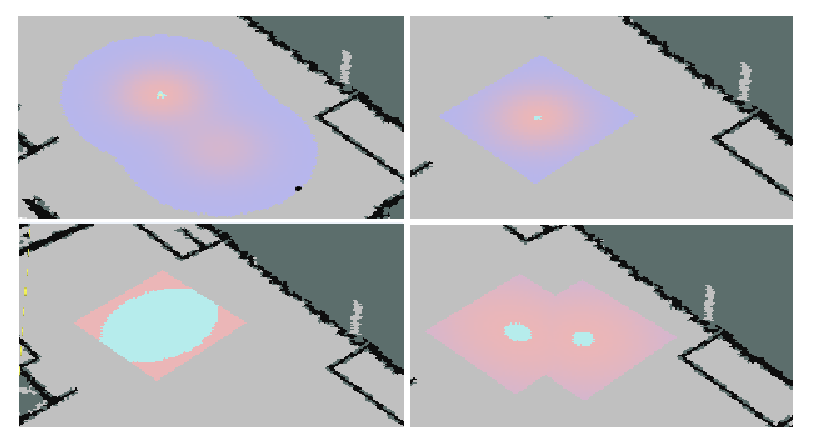
\includegraphics[width=0.37\textwidth]{pictures/all.eps}\label{fig:costmapPic}}%

\caption{Sample costmap shapes. Top left: convolution method, top right: standard 2D Gaussian, bottom left: K-means, and bottom right: mean shift.}
\label{fig:costmapPic}
\end{figure}

%1. FMM + without uncertainity\\2. FMM + with uncertainity\\	2a. Convolution\\	2b. clustering\\3. DWA + without uncertainity\\4. DWA + with uncertainity\\	2a. Convolution\\	2b. clustering\\

%All these should have simulations and real robot experiments.\\
\begin{figure}
%\left
\subfloat[]{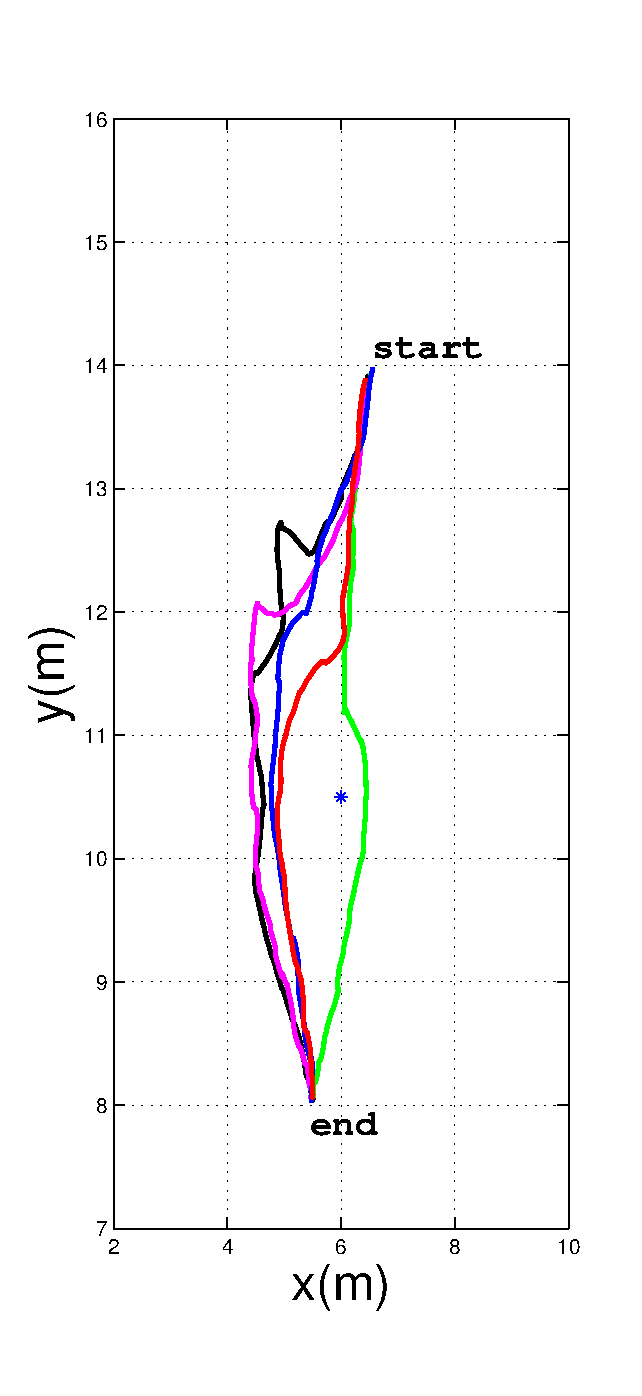
\includegraphics[width=0.168\textwidth, trim= 3mm 12.5mm 0mm 15.5mm, clip]{pictures/traj1.eps}\label{fig:traj1}}%
%\hspace{0.1cm}
\subfloat[]{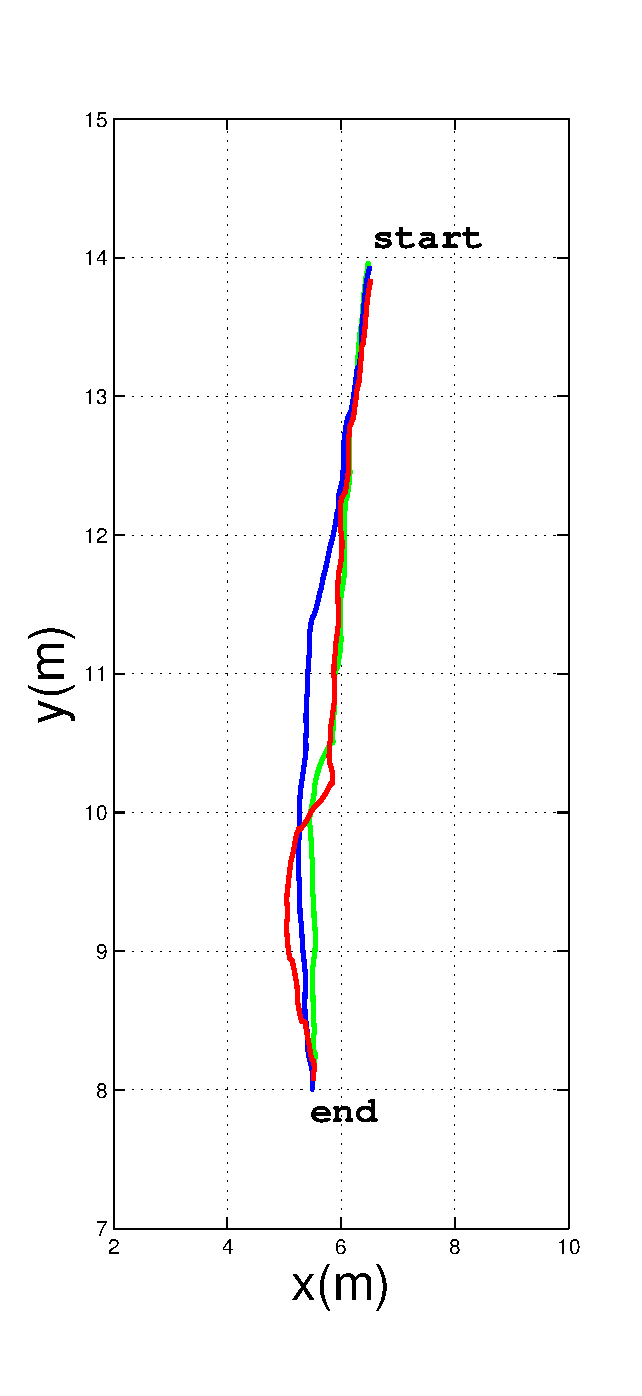
\includegraphics[width=0.168\textwidth, trim= 3mm 6.5mm 0mm 16mm, clip]{pictures/traj2.eps}\label{fig:traj2}}%
%\hspace{0.1cm}
\subfloat[]{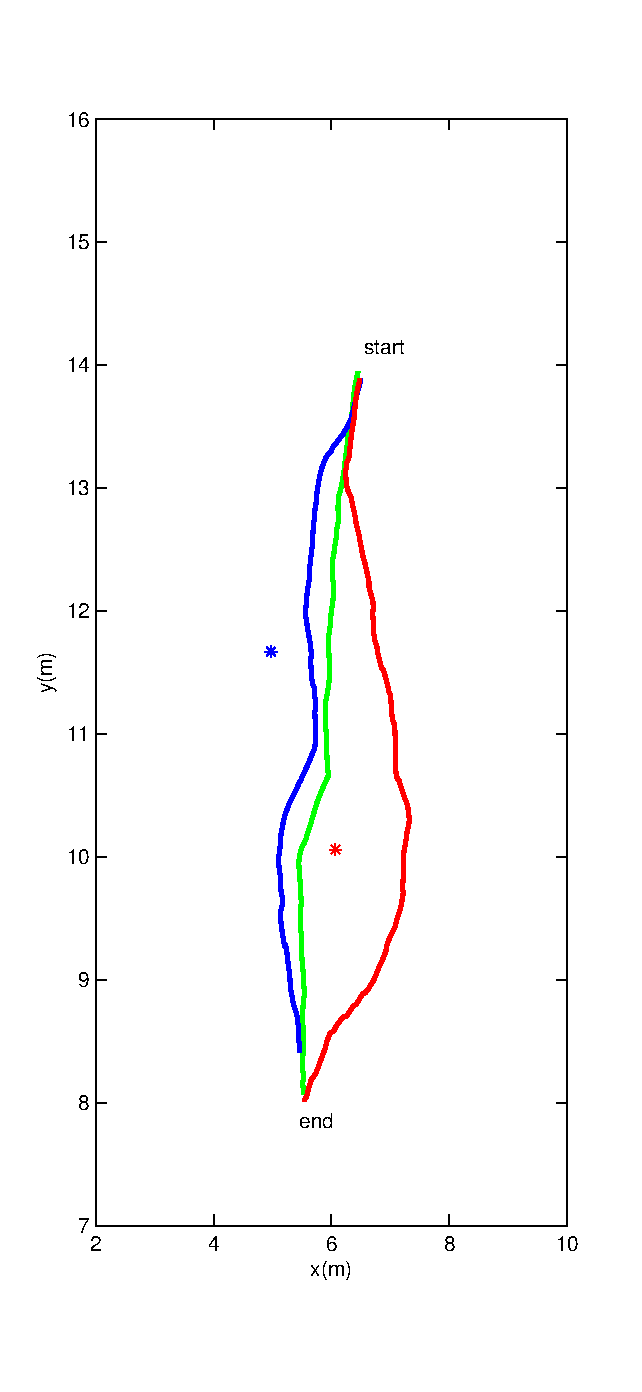
\includegraphics[width=0.168\textwidth, trim= 3mm 12.5mm 0mm 15.5mm, clip]{pictures/traj3.eps}\label{fig:traj3}}%
%\hspace{0.1cm}

\caption{Sample robot trajectories for different methods. Color coding: green for BN, red for DHA, black for KHA, pink for SHA and blue for CHA. Scenarios: (a) Single static person. (b) Single dynamic person. The trajectory of the person is indicated by the dark green dashed line. (c) Two static people. Each circle represents a static person.
%Dots: static people.
}
\label{fig:trajs}
\end{figure}

\begin{figure*}
\centering
\subfloat[]{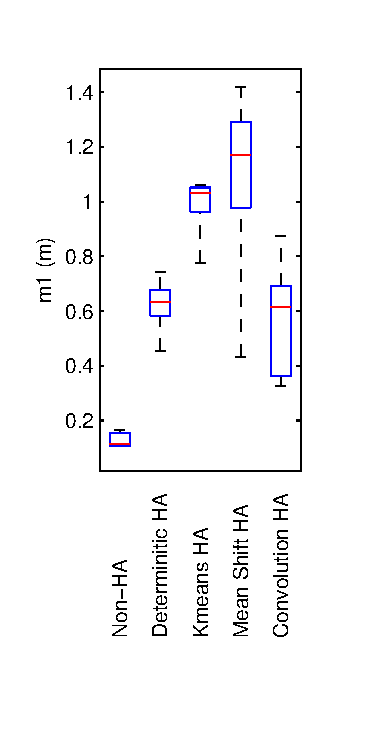
\includegraphics[width=0.168\textwidth, trim= 1mm 13mm 2mm 8mm, clip]{pictures/m1.eps}\label{fig:1_1}}%
%\hspace{%0.1cm}
\subfloat[]{\includegraphics[width=0.1680\textwidth, trim= 1mm 13mm 2mm 8mm, clip]{pictures/m2.eps}\label{fig:1_2}}%
%\hspace{0.1cm}
\subfloat[]{\includegraphics[width=0.1680\textwidth, trim= 1mm 13mm 2mm 8mm, clip]{pictures/m3.eps}\label{fig:1_3}}%
%\hspace{0.1cm}
\subfloat[]{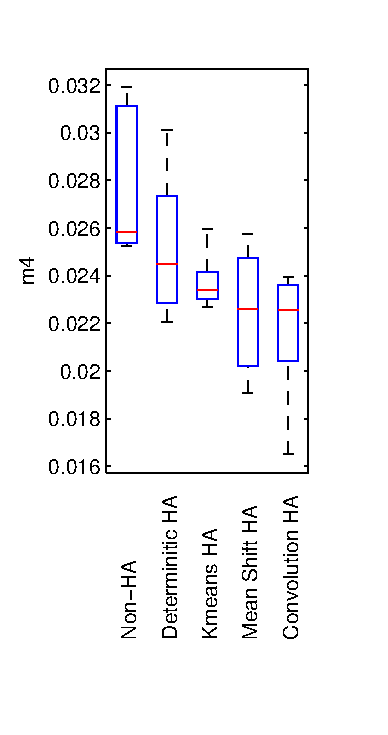
\includegraphics[width=0.1680\textwidth, trim= 1mm 13mm 2mm 8mm, clip]{pictures/m4.eps}\label{fig:1_4}}%
%\hspace{0.1cm}
\subfloat[]{\includegraphics[width=0.168\textwidth, trim= 1mm 13mm 2mm 8mm, clip]{pictures/m5.eps}\label{fig:1_5}}%

\caption{Performance metrics obtained in the single static person scenario. HA stands for Human-Aware in the plot labels.
}
\label{fig:boxplots_singlePerson}
\end{figure*}

\subsection{Results}
\label{sec:results}
Figure \ref{fig:costmapPic} shows sample costmaps of the different methods mentioned earlier. It can be seen that the clustering methods can end up with wrong number of clusters or saturated costs when the uncertainty is high due to large $\sigma$ values. The convolution costmap has a much more flexible shape and is not limited whereas other costmaps all have a cut off distance.

Sample trajectories of the robot are depicted in Fig. \ref{fig:trajs}. It is clear from the plots that HA methods result in trajectories that preserve larger distances to the people.
%Larger distance for BN compared to CHA to the red person in \ref{fig:traj3} is due to the robot being ignorant of that person and trying to move in a straight line towards the goal. 
Additionally, they are smoother and therefore more natural from the point of view of a person, this is supported by Fig. \ref{fig:1_4}, \ref{fig:2_2}, and \ref{fig:3_4}. However, this may not be evident from the trajectory plots. This is due to the abrupt movement of non-HA navigation upon encountering a person which considerably affects the smoothness.

Clustering methods can cause the robot to modify its plan largely by enforcing a certain cluster shape upon finding cluster centroids: if the new probabilistic data leads to a new centroid that is not very close to the previous one, the costmap could change significantly and thus the planned path. This is more severe for mean shift clustering due to adaptively modifying the number of clusters as well. This is to be expected given the probabilistic nature of the perception data, however the plan can be modified more smoothly using the convolution method. This method which outperforms all other methods in terms of smoothness in all of our tests, is shown to be a remedy to this problem based on our experimental results. Hence, for the second and third scenario, we only compare the results of BN, DHA, and CHA methods.  

When comparing the results of DHA with CHA we can see that the former is a more conservative method in terms of keeping distance to the people when receiving accurate data. If DHA receives a perfect estimate of the person's position it can lead to the desired path; however, this is seldom the case. Particularly, in the case of a moving person, the detector could not always keep up with the speed of the person, \textit{i.e.}, the position estimates were reported with delay or the person was lost in some cases, and the robot was faced with the human while considering him an obstacle. This led to abrupt changes and getting too close to the person, see Fig.~\ref{fig:traj2}. However, by associating larger uncertainty to the estimates in this case, CHA could lead to better plans in terms of proximity and smoothness. Unfortunately, due to our inaccurate ground truth of the moving person, we only rely on $m_{4}$ and $m_{5}$ for scenario 2, but we observed the delayed perception and lost person problem during our experiments. 




\begin{figure}
\centering
\subfloat[]{\includegraphics[width=0.1490\textwidth, trim= 0mm 13mm 2mm 8mm, clip]{pictures/dy_m4.eps}\label{fig:2_2}}%
\hspace{0.1cm}
\subfloat[]{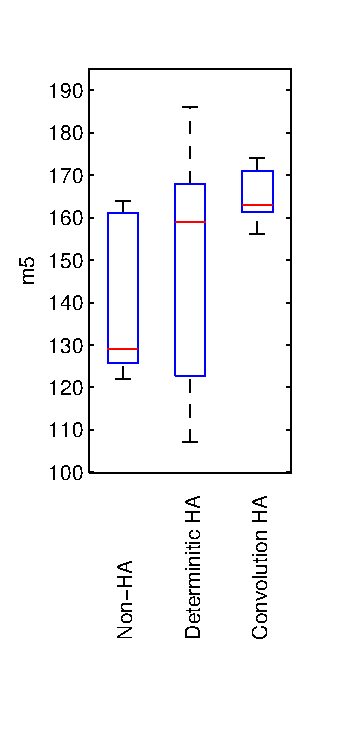
\includegraphics[width=0.149\textwidth, trim= 0mm 13mm 2mm 8mm, clip]{pictures/dy_m5.eps}\label{fig:2_3}}%

\caption{Performance metrics obtained in the dynamic person scenario. %HA stands for Human-Aware in the plot labels.
}
\label{fig:boxplots_singlePersonMov}
\end{figure}

%
\begin{figure}
\centering
\subfloat[]{\includegraphics[width=0.162\textwidth, trim= 1mm 13mm 2mm 8.5mm, clip ]{pictures/two_m1.eps}\label{fig:3_1}}% \vspace{<whatever>}
%\hspace{0.1cm}
\subfloat[]{\includegraphics[width=0.162\textwidth, trim= 1mm 13mm 2mm 8.5mm, clip ]{pictures/two_m2.eps}\label{fig:3_2}}%
%\hspace{0.1cm}
\subfloat[]{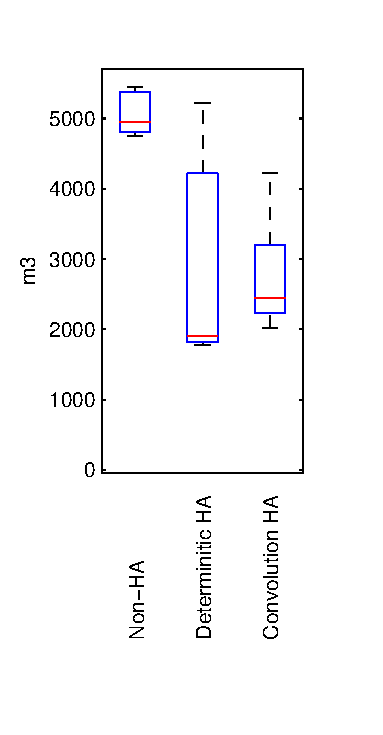
\includegraphics[width=0.162\textwidth, trim= 1mm 13mm 2mm 8.5mm, clip ]{pictures/two_m3.eps}\label{fig:3_3}}%

%\hspace{0.1cm}
\subfloat[]{\includegraphics[width=0.162\textwidth, trim= 1mm 13mm 2mm 8.5mm, clip ]{pictures/two_m4.eps}\label{fig:3_4}}%
%\hspace{0.1cm}
\subfloat[]{\includegraphics[width=0.162\textwidth, trim= 1mm 13mm 2mm 8.5mm, clip ]{pictures/two_m5.eps}\label{fig:3_5}}%
%\hspace{0.1cm}
%\subfloat[]{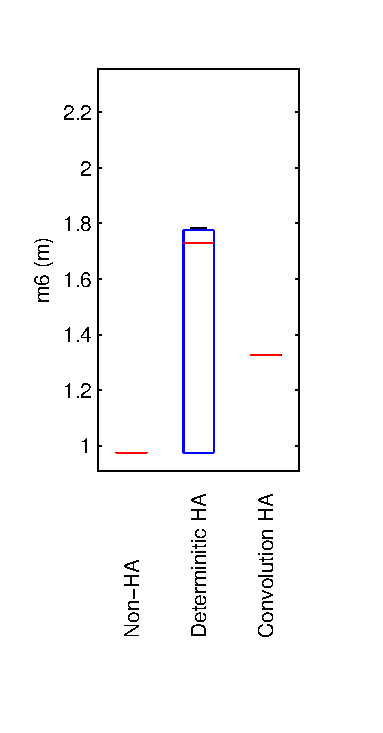
\includegraphics[width=0.163\textwidth, trim= 2mm 13mm 2mm 8mm, clip ]{pictures/two_m6.eps}\label{fig:3_6}}%

\caption{Performance metrics obtained in the two static people scenario.
% HA stands for Human-Aware in the plot labels.
}
\label{fig:boxplots_2people}
\end{figure}


Figures \ref{fig:boxplots_singlePerson}, \ref{fig:boxplots_singlePersonMov} and \ref{fig:boxplots_2people} show the performance metrics for the three scenarios. We will discuss the results of each metric in the following. $m_{1}$ has increased for HA methods which shows the effectiveness of our FMM planner in social path planning. However, DHA is more conservative in this regard in the presence of good perception data. $m_{2}$ has increased for uncertainty-based methods in the simple scenario as the deterministic tracker is giving already good position estimates, but this is no longer the case when the complexity is increased as seen in Fig. \ref{fig:3_2}. $m_{3}$ is also reduced for HA methods and more so for uncertainty-based HA methods considering all trials, as the complexity of the problem increases, see Fig.\ref {fig:3_3}.


$m_{4}$ is showing a very interesting result, we can see how uncertainty-based HA methods have managed to introduce smoothness into the trajectories by reducing jerk without deliberately accounting for it. CHA is dominating other methods across all scenarios in this case. Lastly, $m_{5}$ which shows the total navigation time is always lower for BN due to optimizing the path length only. The largest values belong to KHA and SHA due to constant modifications of the path, thus taking longer routes. For DHA this metric is lower than CHA for the static person case and comparable to CHA in the moving person scenario, but it increases as the complexity of the environment grows further in the case of multiple people.% Lastly, $m_{6}$ which is only used in the third scenario, indicates how DHA has varying behavior (sometimes takes a detour) based on the tracker estimates whereas CHA has more or less the same behavior in our runs due to its probabilistic nature when computing the social costmap.     



%\subsection{Discussion}
%\label{sec:discussion}

\section{Conclusion and future work}
\label{sec:conclusion}

In this work we have proposed a novel approach for extending the model of social costmaps to include uncertainty of perception. Experiments show how this extended model can lead to more natural robot trajectories that preserve a social distance from people. By combining the output of a probabilistic MCMC-based tracker with an expectation costmap computation method based on convolution, we introduce a principled approach to solve the social path planning problem in real environments with multiple people while explicitly dealing with perception uncertainty. 



The idea presented in this paper can be extended to other types of perception sources. By providing probabilistic perception outputs, the proposed model can fulfill this task without loss of performance, since the probabilistic language provides a common ground to quantitatively express uncertainty regardless of the type of the sensor. 


Further improvements can be made to the accuracy of robot self-localization and the ground truth of people positions, as they have direct influence on performance evaluations. Moreover, quantifying the uncertainty of perception (investigating the impact of different levels of perception uncertainty on the behavior and performance of each part of our system) can be useful in analyzing the behavior of expectation-based social costmap computation methods for further in-depth studies.


As a future step for this research, we plan to test our approach with multiple perception sources with different uncertainties, particularly on-board perception which allows for much more flexibility in terms of applications and fewer physical limitations.% Another interesting area of exploration is replanning, \textit{i.e.}, what replanning strategy works best for a real dynamic social environment.

%Currently, replanning is done upon a change in the costmap but this is not necessarily the best strategy. It would be interesting to investigate the effect of local and global path planners along with different replanning strategies on human-aware navigation.  





%\section*{Acknowledgements}

%This work has been supported by the European MOnarCH project FP7-ICT-9-2011-601033. 





% \addtolength{\textheight}{-12cm}   % This command serves to balance the column lengths
                                  % on the last page of the document manually. It shortens
                                  % the textheight of the last page by a suitable amount.
                                  % This command does not take effect until the next page
                                  % so it should come on the page before the last. Make
                                  % sure that you do not shorten the textheight too much.

%%%%%%%%%%%%%%%%%%%%%%%%%%%%%%%%%%%%%%%%%%%%%%%%%%%%%%%%%%%%%%%%%%%%%%%%%%%%%%%%

% \section*{APPENDIX}
% Appendixes should appear before the acknowledgment.

%\section*{Acknowledgement}
%This research was supported by the Swiss National Science Foundation through the National Center of Competence in Research Robotics.
% The preferred spelling of the word �acknowledgment� in America is without an �e� after the �g�. Avoid the stilted expression, �One of us (R. B. G.) thanks . . .�  Instead, try �R. B. G. thanks�. Put sponsor acknowledgments in the unnumbered footnote on the first page.

%\begin{thebibliography}{99}
%\end{thebibliography}

%Equalize columns in last page
\IEEEtriggeratref{11}

\bibliographystyle{IEEEtran}
\bibliography{papers}

\end{document}
